\documentclass[10pt,a4paper]{article}

\usepackage[a4paper,margin=0.62in]{geometry}
\usepackage{graphicx}
\usepackage{booktabs}
\usepackage{float}
\usepackage{enumitem}
\usepackage{titlesec}
\usepackage{hyperref}
\usepackage{caption}

\setlength{\parindent}{0pt}
\setlength{\parskip}{0.25em}
\setlist{nosep,leftmargin=1.4em}

\captionsetup{font=small,labelfont=bf}

\titleformat{\section}
  {\large\bfseries}
  {\thesection.}
  {0.4em}
  {}

\titleformat{\subsection}
  {\normalsize\bfseries}
  {\thesubsection.}
  {0.4em}
  {}

\titlespacing*{\section}{0pt}{0.45em}{0.2em}
\titlespacing*{\subsection}{0pt}{0.3em}{0.15em}

\hypersetup{
    colorlinks=true,
    urlcolor=blue,
    linkcolor=black
}

\begin{document}

% =========================================================
% PAGE 1
% =========================================================

\begin{center}
    {\Large\bfseries CSC3173: Artificial Intelligence (2024/25)}\\[0.25em]
    {\large\bfseries Programming Assignment 01}\\[0.35em]
    {\Large\bfseries Customer Churn Prediction: XGBoost vs MLP}\\[0.35em]
    \textbf{Registration Number: S/21/513}
\end{center}

\vspace{-0.35em}

\section{Introduction}

Customer churn prediction is a binary-classification task used to identify customers who are likely to discontinue a service. This assignment compares \textbf{XGBoost} and a \textbf{Multilayer Perceptron (MLP)} using the IBM Telco Customer Churn dataset. Performance is evaluated using \textbf{Accuracy, Precision, Recall, and F1-score}. Since the dataset is imbalanced, Recall and F1-score are particularly useful for evaluating churn detection.

\section{Dataset and Preprocessing}

The dataset contains \textbf{7,043 customer records} and \textbf{33 original columns}. The target variable is \texttt{Churn Value}, where 0 represents no churn and 1 represents churn. The dataset contains 5,174 non-churn customers (73.46\%) and 1,869 churn customers (26.54\%).

Columns that could cause target leakage or provide unnecessary identifier/location information were removed. These included \texttt{CustomerID}, location-related fields, \texttt{Churn Label}, \texttt{Churn Score}, \texttt{CLTV}, and \texttt{Churn Reason}. The \texttt{Total Charges} column was converted to numeric form, and 11 missing values were replaced using the median.

The final dataset contained \textbf{19 predictor variables}: 16 categorical and 3 numerical. Categorical variables were one-hot encoded, while numerical variables were standardized using \texttt{StandardScaler}. An 80:20 stratified train/test split was used with \texttt{random\_state=42}. After preprocessing, the input contained \textbf{46 features}.

\section{Implementation Environment}

The experiment was implemented using Python 3.12 in a \texttt{uv}-managed virtual environment and executed in JupyterLab.

\begin{figure}[H]
    \centering
    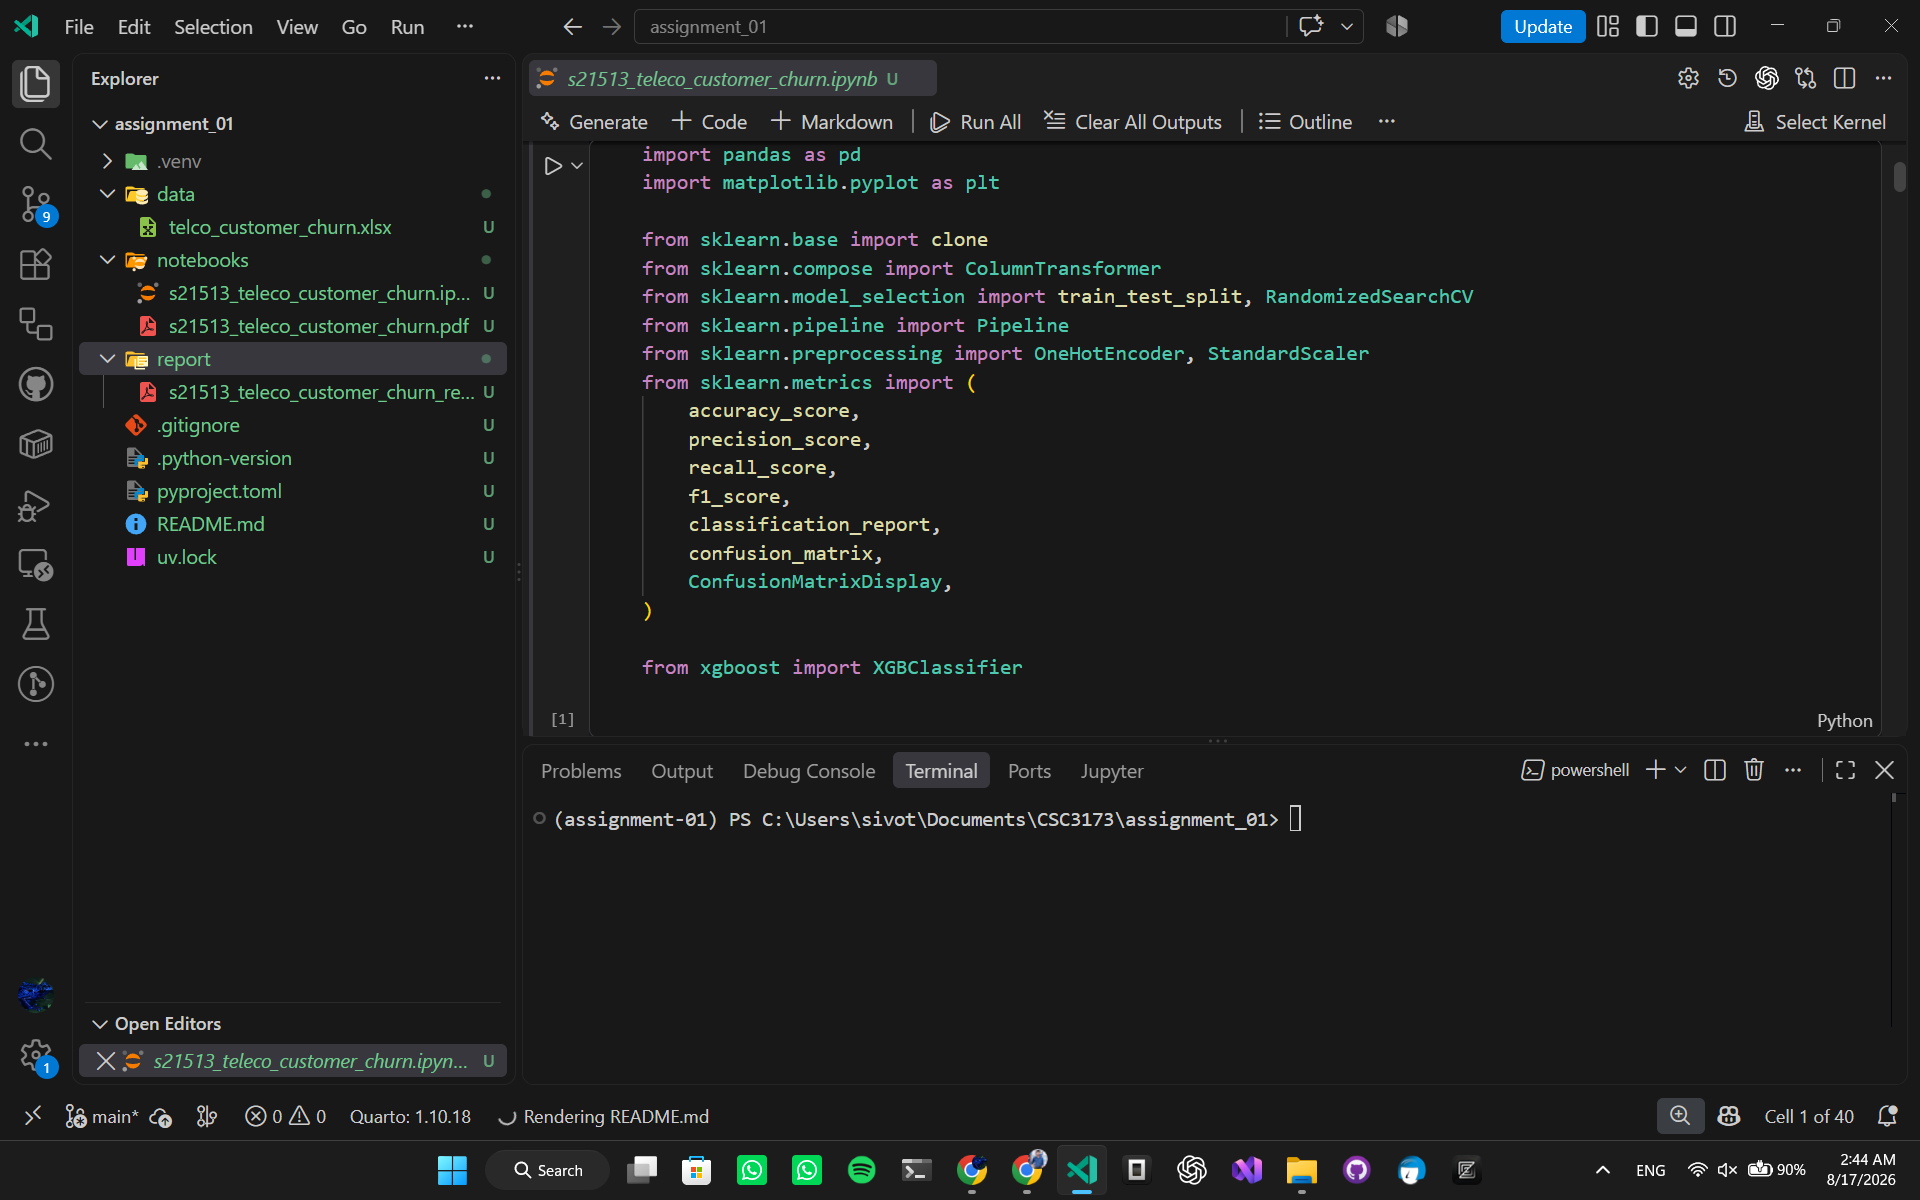
\includegraphics[
        width=2\linewidth,
        height=10cm,
        keepaspectratio
    ]{screenshots/environment.png}
    \caption{Development environment used to execute the assignment.}
\end{figure}

\newpage

% =========================================================
% PAGE 2
% =========================================================

\section{XGBoost Classifier}

\subsection{Baseline XGBoost}

A baseline \texttt{XGBClassifier} was trained using the preprocessed training data.

\begin{table}[H]
\centering
\caption{Baseline XGBoost performance}
\begin{tabular}{lc}
\toprule
\textbf{Metric} & \textbf{Score} \\
\midrule
Accuracy  & 0.7892 \\
Precision & 0.6207 \\
Recall    & 0.5294 \\
F1-score  & 0.5714 \\
\bottomrule
\end{tabular}
\end{table}

\subsection{Hyperparameter Optimization}

Hyperparameter optimization was performed using \texttt{RandomizedSearchCV}. A 5-fold cross-validation strategy was applied to the training set, and F1-score was used as the optimization criterion. Thirty parameter combinations were evaluated, resulting in 150 model fits.

\begin{table}[H]
\centering
\caption{Best XGBoost hyperparameters}
\begin{tabular}{lc}
\toprule
\textbf{Hyperparameter} & \textbf{Best Value} \\
\midrule
\texttt{n\_estimators}      & 200 \\
\texttt{max\_depth}         & 3 \\
\texttt{learning\_rate}     & 0.05 \\
\texttt{subsample}          & 0.9 \\
\texttt{colsample\_bytree}  & 0.8 \\
\texttt{min\_child\_weight} & 5 \\
\bottomrule
\end{tabular}
\end{table}

The best cross-validation F1-score was \textbf{0.6142}.

\begin{table}[H]
\centering
\caption{Optimized XGBoost performance}
\begin{tabular}{lc}
\toprule
\textbf{Metric} & \textbf{Score} \\
\midrule
Accuracy  & 0.8070 \\
Precision & 0.6656 \\
Recall    & 0.5481 \\
F1-score  & 0.6012 \\
\bottomrule
\end{tabular}
\end{table}

Hyperparameter optimization improved all four reported metrics compared with the baseline XGBoost model.

\begin{figure}[H]
    \centering
    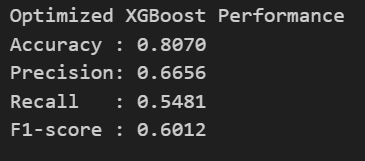
\includegraphics[
        width=1\linewidth,
        height=6cm,
        keepaspectratio
    ]{screenshots/xgboost_output.png}
    \caption{Sample XGBoost code and generated performance output.}
\end{figure}

\newpage

% =========================================================
% PAGE 3
% =========================================================

\section{Multilayer Perceptron (MLP)}

\subsection{Baseline MLP}

The baseline MLP consisted of two hidden ReLU layers containing 64 and 32 neurons, followed by a single sigmoid output neuron. The model used the Adam optimizer, binary cross-entropy loss, batch size 32, and early stopping based on validation loss.

\begin{table}[H]
\centering
\caption{Baseline MLP performance}
\begin{tabular}{lc}
\toprule
\textbf{Metric} & \textbf{Score} \\
\midrule
Accuracy  & 0.7828 \\
Precision & 0.5813 \\
Recall    & 0.6497 \\
F1-score  & 0.6136 \\
\bottomrule
\end{tabular}
\end{table}

\subsection{Hyperparameter Optimization}

For MLP hyperparameter selection, the original training set was divided into internal training and validation subsets. Candidate models varied hidden-layer size, learning rate, dropout rate, and batch size. Validation F1-score was used to select the best configuration.

\begin{table}[H]
\centering
\caption{Best MLP hyperparameters}
\begin{tabular}{lc}
\toprule
\textbf{Hyperparameter} & \textbf{Best Value} \\
\midrule
First hidden layer  & 64 neurons \\
Second hidden layer & 32 neurons \\
Learning rate       & 0.0005 \\
Dropout rate        & 0.3 \\
Batch size          & 32 \\
Epochs              & 27 \\
\bottomrule
\end{tabular}
\end{table}

The best validation F1-score was \textbf{0.6484}. A fresh MLP was then trained on the full training set using the selected configuration.

\begin{table}[H]
\centering
\caption{Optimized MLP performance}
\begin{tabular}{lc}
\toprule
\textbf{Metric} & \textbf{Score} \\
\midrule
Accuracy  & 0.8013 \\
Precision & 0.6655 \\
Recall    & 0.5053 \\
F1-score  & 0.5745 \\
\bottomrule
\end{tabular}
\end{table}

Although tuning improved MLP accuracy and precision, Recall and F1-score decreased on the final test set.

\begin{figure}[H]
    \centering
    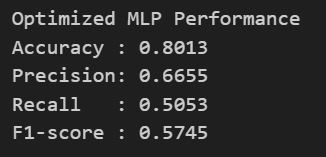
\includegraphics[
        width=1\linewidth,
        height=6cm,
        keepaspectratio
    ]{screenshots/mlp_output.png}
    \caption{Sample MLP code and generated performance output.}
\end{figure}

\newpage

% =========================================================
% PAGE 4
% =========================================================

\section{Final Performance Comparison}

\begin{table}[H]
\centering
\caption{Performance comparison of all models}
\small
\begin{tabular}{lcccc}
\toprule
\textbf{Model} &
\textbf{Accuracy} &
\textbf{Precision} &
\textbf{Recall} &
\textbf{F1-score} \\
\midrule
XGBoost Baseline & 0.7892 & 0.6207 & 0.5294 & 0.5714 \\
XGBoost Tuned    & \textbf{0.8070} & \textbf{0.6656} & 0.5481 & 0.6012 \\
MLP Baseline     & 0.7828 & 0.5813 & \textbf{0.6497} & \textbf{0.6136} \\
MLP Tuned        & 0.8013 & 0.6655 & 0.5053 & 0.5745 \\
\bottomrule
\end{tabular}
\end{table}

\section{Discussion}

The tuned XGBoost model achieved the highest \textbf{accuracy (0.8070)} and \textbf{precision (0.6656)}. Hyperparameter tuning increased its F1-score from 0.5714 to 0.6012.

The baseline MLP achieved the highest \textbf{recall (0.6497)} and \textbf{F1-score (0.6136)}, indicating that it identified a larger proportion of customers who actually churned. In a customer-retention application, Recall is important because a false negative represents a churn customer who was not detected.

The tuned MLP achieved relatively high accuracy and precision but lower Recall and F1-score than the baseline MLP. This result demonstrates the importance of evaluating the selected model on an untouched test set instead of relying only on validation performance.

\begin{figure}[H]
    \centering
    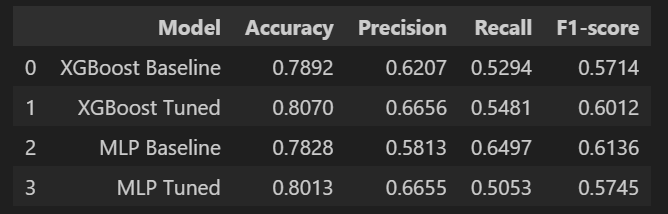
\includegraphics[
        width=2\linewidth,
        height=5cm,
        keepaspectratio
    ]{screenshots/confusion_matrices.png}
    \caption{Confusion matrices for the tuned XGBoost and MLP models.}
\end{figure}

\section{Conclusion}

Both XGBoost and MLP were successfully applied to customer churn prediction. The \textbf{tuned XGBoost} model was strongest when Accuracy and Precision were prioritized, while the \textbf{baseline MLP} achieved the highest Recall and F1-score.

Therefore, tuned XGBoost is preferable when predictive correctness and precision are the main objectives, whereas the baseline MLP is preferable when identifying a larger proportion of actual churn customers is more important.

\section*{References}

\begin{enumerate}
    \item IBM Telco Customer Churn Dataset. \textit{Kaggle}.\\
    \url{https://www.kaggle.com/datasets/yeanzc/telco-customer-churn-ibm-dataset}

    \item Project source code. \textit{GitHub}.\\
    \url{https://github.com/sivothajan/s21513_csc3173_teleco_customer_churn}
\end{enumerate}

\end{document}
